% RQ3 explanation-aware alpha-sweep. Compile from this folder:
%   pdflatex -interaction=nonstopmode -halt-on-error -output-directory=../Figures fig_alpha_sweep.tex
% Include in main.tex:
%   
\includegraphics[width=0.8\linewidth]{Figures/fig_alpha_sweep}
%
% B&W-friendly (professor's rule): the three data series are distinguished by
% MARKER SHAPE and LINE STYLE, not by colour. All data is ink-black; grey is used
% only for the random-choice guide line.
\documentclass[tikz,border=7pt]{standalone}
\usepackage[scaled=0.95]{helvet}
\renewcommand{\familydefault}{\sfdefault}
\usepackage{amsmath}
\usepackage{pgfplots}
\pgfplotsset{compat=1.16}
\usepackage{xcolor}

\definecolor{ink}{HTML}{1F2933}
\definecolor{muted}{HTML}{5B6776}
\definecolor{line}{HTML}{9AA7B5}
\definecolor{accent}{HTML}{255E88}

\begin{document}
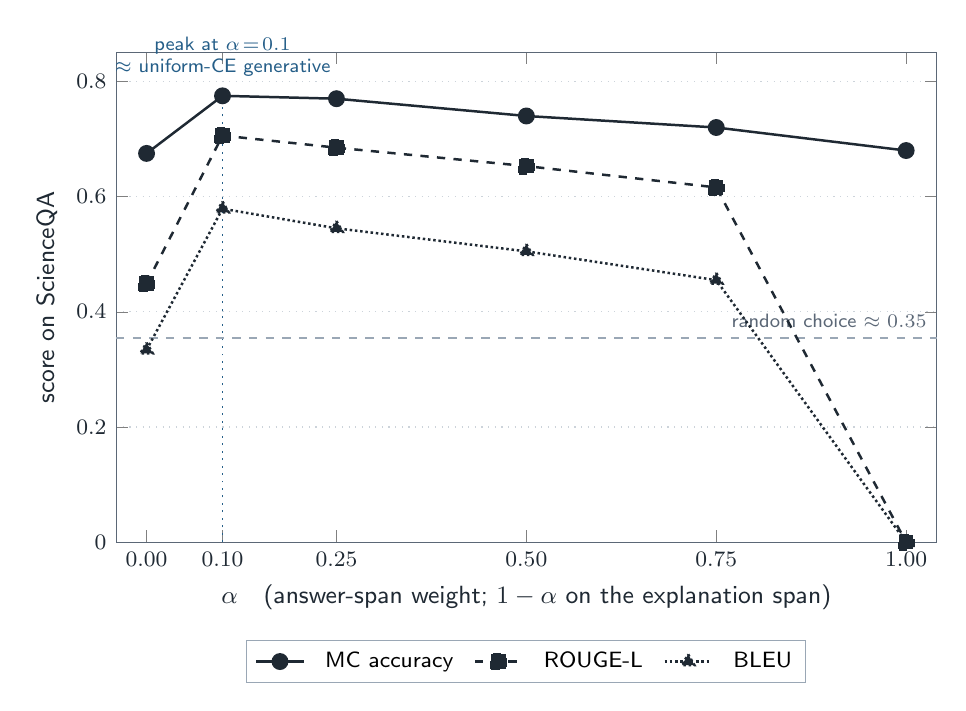
\begin{tikzpicture}[font=\sffamily\small]
\begin{axis}[
  width=12cm, height=7.8cm,
  xlabel={$\alpha$\quad(answer-span weight; $1-\alpha$ on the explanation span)},
  ylabel={score on ScienceQA},
  xmin=-0.04, xmax=1.04,
  ymin=0, ymax=0.85,
  xtick={0,0.1,0.25,0.5,0.75,1.0},
  ytick={0,0.2,0.4,0.6,0.8},
  xticklabel style={/pgf/number format/.cd, fixed, fixed zerofill, precision=2},
  ymajorgrids=true,
  grid style={line!50, dotted},
  axis line style={muted},
  tick label style={text=ink, font=\footnotesize},
  label style={text=ink},
  legend cell align={left},
  legend style={draw=line, font=\footnotesize, at={(0.5,-0.20)}, anchor=north,
                legend columns=3, column sep=1.2ex},
  every axis plot/.append style={line width=0.9pt, mark size=2.6pt},
  clip=false,
]

% random-choice baseline (grey guide, not a data series)
\addplot[line, dashed, line width=0.6pt, forget plot]
  coordinates {(-0.04,0.354) (1.04,0.354)};
\node[muted, font=\scriptsize, anchor=south east] at (axis cs:1.04,0.356)
  {random choice $\approx 0.35$};

% MC accuracy --- solid, filled circle
\addplot[ink, mark=*, mark options={fill=ink}] coordinates {
  (0,0.675) (0.1,0.775) (0.25,0.770) (0.5,0.740) (0.75,0.720) (1.0,0.680)};
\addlegendentry{MC accuracy}

% ROUGE-L --- dashed, filled square
\addplot[ink, dashed, mark=square*, mark options={fill=ink}] coordinates {
  (0,0.449) (0.1,0.706) (0.25,0.685) (0.5,0.653) (0.75,0.616) (1.0,0.000)};
\addlegendentry{ROUGE-L}

% BLEU --- dotted, filled triangle
\addplot[ink, densely dotted, mark=triangle*, mark options={fill=ink}] coordinates {
  (0,0.334) (0.1,0.579) (0.25,0.545) (0.5,0.505) (0.75,0.455) (1.0,0.000)};
\addlegendentry{BLEU}

% annotate the interior optimum / generative coincidence
\node[accent, font=\scriptsize, anchor=south, align=center]
  at (axis cs:0.10,0.792) {peak at $\alpha\!=\!0.1$\\$\approx$ uniform-CE generative};
\draw[accent, line width=0.7pt, dotted] (axis cs:0.1,0) -- (axis cs:0.1,0.775);

\end{axis}
\end{tikzpicture}
\end{document}
